\subsection{Electromagnetic calorimeter}
\label{sec:ecal}

The CMS electromagnetic calorimeter (ECAL)
\nomenclature{ECAL}{Electromagnetic calorimeter} 
is a hermetic, homogenous calorimeter made of 
lead tungstate ($\text{PbWO}_4$) crystals.  
Its purpose is to provide a high resolution measurement 
of the energy of electromagnetic showers.
The ECAL 
is split into two subdetectors consisting of a barrel 
region (EB)
\nomenclature{EB}{Electromagnetic calorimeter barrel}
and two endcap regions (EE).
\nomenclature{EE}{Electromagnetic calorimeter endcap}
In addition, a preshower detector (ES) 
\nomenclature{ES}{Electromagnetic calorimeter preshower}
made of silicon strips is placed in front of the endcaps to identify
neutral pions in the high pseudorapidity region.
A schematic cross section of the ECAL is shown in Figure \ref{fig:ecal}.

\begin{figure}
  \centering
  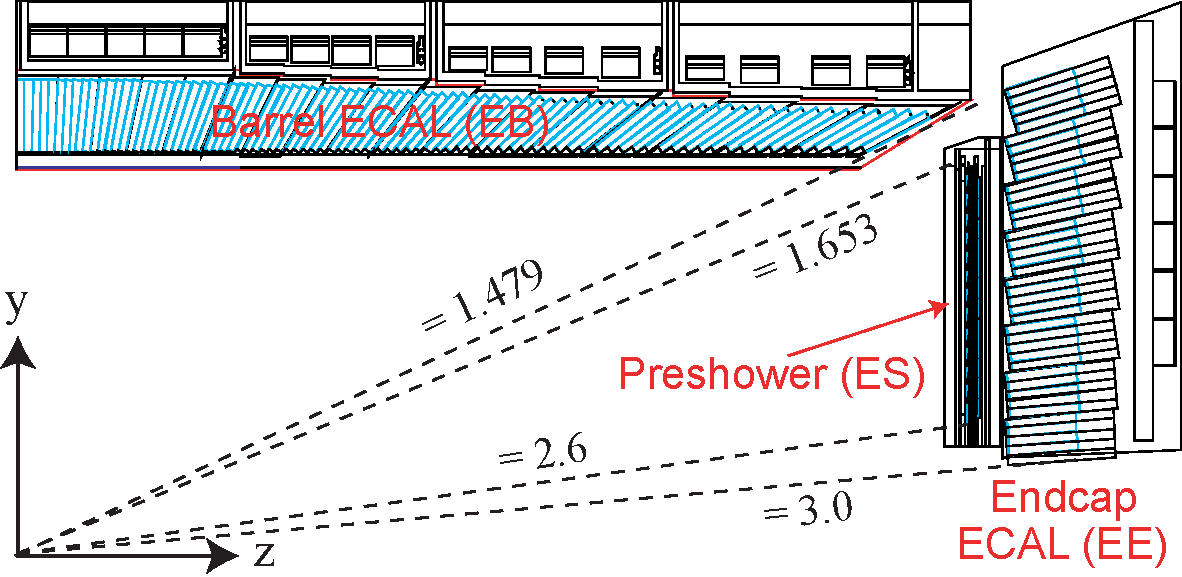
\includegraphics[width=1.0\textwidth]{tex/cms/fig/ecal-schematic-2.pdf}
  \caption{A schematic cross section of the CMS ECAL.  Only one quarter of the entire
    ECAL is represented. The three subsystems of the ECAL: the barrel (EB), endcap (EE),
    and preshower (ES) are all shown. \cite{cms-tdr}}
  \label{fig:ecal}
\end{figure}


\begin{table}
  \centering
  \begin{tabular}{c|c}
    Property & Value \\
    \hline\hline
    Chemical composition & Lead tungstate crystal ($\text{PbWO}_4$) \\
    Density & 8.28 $\text{g}/\text{cm}^{3}$ \\
    Radiation length & 0.89 cm \\
    Interaction length & 19.5 cm \\
    Moli\`{e}re radius & 2.2 cm \\
  \end{tabular}
  \caption{Properties of the EB and EE scintillating crystals \cite{cms-jinst}.}
  \label{tab:ecal-crystal}
\end{table}

Lead tungstate crystals have a 
high density,
a short radiation length,
and a small Moli\`{e}re radius,
which allow for a compact calorimeter with fine granularity. 
The numeric values for these parameters are given in Table \ref{tab:ecal-crystal}.
They are also optically clear and radiation resistant.
The crystals scintillate with a relatively low light output
that varies with temperature: maximum output is 4.5 photoelectrons
per MeV at $18^{\circ}{\rm C}$, and the output declines from that maximum at $-2.1\%/^{\circ}{\rm C}$.
The scintillation decay time is roughly the same as the LHC bunch crossing
length: $80\%$ of the light is emitted in 25 ns.  
The light output is blue-green with a broad maximum at 420-430 nm, and it is
collected by avalanche photodiodes (APDs)
\nomenclature{APD}{Avalanche photodiode} in the EB and
vacuum phototriodes (VPTs) 
\nomenclature{VPT}{Vacuum phototriode} in the EE.
Photographs of lead tungstate crystals with photodetectors attached 
are shown in Figure \ref{fig:ecal-crystal}.

\begin{figure}
  \centering
  \begin{subfigure}[b]{0.49\textwidth}
    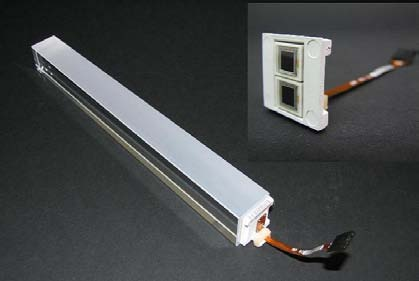
\includegraphics[width=\textwidth]{tex/cms/fig/ecal-crystal-eb.jpg}
    \caption{}
    \label{fig:ecal-crystal-eb}
  \end{subfigure}
  \begin{subfigure}[b]{0.49\textwidth}
    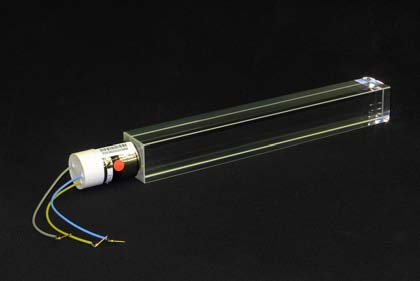
\includegraphics[width=\textwidth]{tex/cms/fig/ecal-crystal-ee.jpg}
    \caption{}
    \label{fig:ecal-crystal-ee}
  \end{subfigure}
  \caption{
    Lead tungstate crystals with photodetectors attached.  The crystal in Figure (a) 
    is a barrel crystal with one face depolished and an APD capsule attached.  
    An APD capsule with two APDs is shown in the inset.
    The crystal in Figure (b) is an endcap crystal with all sides polished and a VPT
    attached \cite{cms-jinst}.
  }
  \label{fig:ecal-crystal}
\end{figure}

The EB covers the pseudorapidity range $|\eta| < 1.479$.  The granularity
of the crystals in the EB is 360-fold in $\phi$ and $2\times85$-fold in $\eta$, 
resulting in a total of 61,200 crystals in the EB.  The crystals themselves
are mounted in a quasi-projective geometry in order to avoid cracks with the
same trajectory as incident particles from the IP.  The crystals have a tapered,
pyramidal shape: the front face has a cross section of $22\times22$ $\text{mm}^2$,
the rear face has a cross section of $26\times26$ $\text{mm}^2$, and the total
length is 230 mm (25.8 $X_0$).  The crystals are arranged into a thin-walled
aveolar structure (submodule).  Each submodule is placed into modules of
different types, depending on pseudorapidity positioning.  Each module 
contains 400 or 500 crystals.  Four modules separated by 4 mm thick aluminum 
webs make a supermodule, which contains 1700 crystals.  The entire EB is
composed of 36 supermodules.

The EE covers the pseudorapidity range $1.479 <|\eta| < 3.0$, and the longitudinal 
distance between the IP and the EE is 3144 mm.  
All of the crystals are laid out in a rectangular $x-y$ grid with 
a quasi-projective geometry.  As in the EB, the crystals have a tapered, pyramidal shape.
In the case of the EE, the front face cross section is $28.62\times28.62$ $\text{mm}^2$,
the read face cross section is $30\times30$ $\text{mm}^2$, and the total length is
220 mm (24.7 $X_0$).
The EE crystals are all identically shaped and are 
arranged into groups of $5\times5$ crystals called supercrystals.
Each endcap is made of two halves called Dees, which each have 138 full supercrystals
and 18 partial supercrystals on the curved inner and outer edge of the Dee.
There are 3662 crystals in each of the four Dees, making a total of 14,648 crystals
in the entire EE.

\begin{figure}
  \centering
  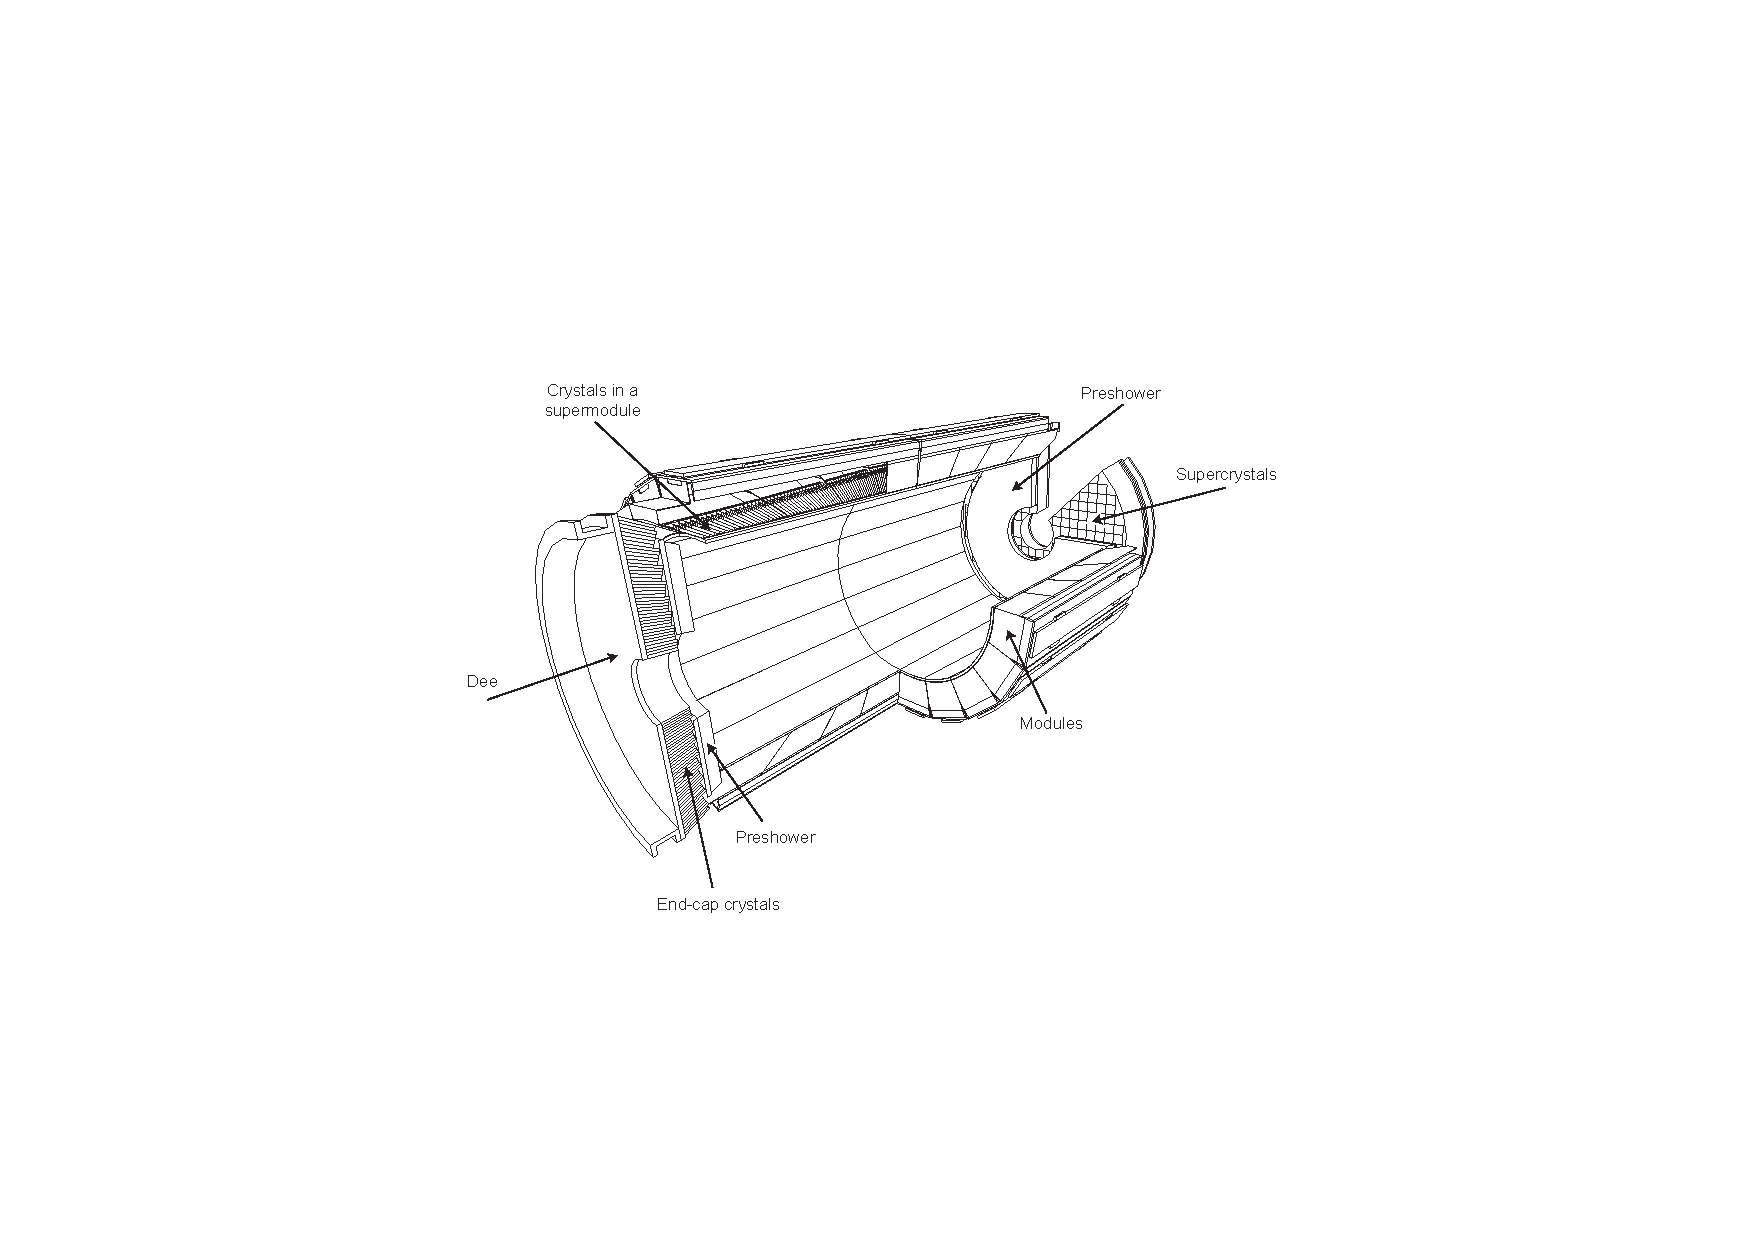
\includegraphics[width=1.0\textwidth]{tex/cms/fig/ecal-schematic.pdf}
  \caption{A three dimensional schematic of the CMS ECAL, showing the positioning 
    of the modules, supermodules, supercrystals, and Dees as described in Section 
    \ref{sec:ecal} \cite{ecal-resolution}.}
  \label{fig:ecal-3d}
\end{figure}

The ES covers the pseudorapidity region $1.653 < |\eta| < 2.6$ and rests
in front of the EE.  Unlike the EB and EE, 
the ES is a sampling calorimeter made up of two layers of silicon strip sensors 
alternating with two layers of lead absorber.  The total thickness is 20 cm.
Each silicon sensor is $63\times63$  $\text{mm}^2$ with an active area of 
$61\times61$  $\text{mm}^2$ divided into 32 strips, each with a 1.9 mm pitch.
Because the pitch of the ES sensors is so much thinner than the front face of the EE crystals,
the ES has significantly better spatial resolution than the EE alone.
This is necessary to distinguish between single photons and closely-spaced photon pairs
(e.g. from $\pi^0 \rightarrow \gamma\gamma$ decays).
The silicon strip sensors in the first layer are set orthogonally to the strips in the second layer. 
The first and second lead layers have material thicknesses of 2 $X_0$ and 1 
$X_0$, respectively, so that 95\% of the incident photons have begun to shower
before reaching the second sensor layer.  
The ES is divided into four Dees (two Dees per endcap), and the ES Dees
mirror the shape and orientation of the EE Dees.
A schematic of the entire ECAL, including the modules, supermodules, supercrystals, and Dees
as described above may be found in Figure \ref{fig:ecal-3d}.


For electromagnetic shower energies below 500 GeV, where shower leakage from the rear of the 
calorimeter is significant, the ECAL energy resolution 
($\sigma/E$) for a given energy $E$ may be parameterized by 
Equation \ref{eqn:ecal-resolution-1}:
\begin{equation}
  \frac{\sigma(E)}{E} =
  \frac{S}{\sqrt{E}} \oplus
  \frac{N}{E}        \oplus  C
  \label{eqn:ecal-resolution-1}
\end{equation}
where $S$ is the stochastic term,
$N$ is the noise term, and 
$C$ is the constant term.
The stochastic term describes event-to-event fluctuations
in the lateral shower containment, photostatic effects,
and fluctuations in the energy deposited in the ES
absorber (in regions where the ES is present) with respect
to the energy measured by the ES silicon.
The noise term describes noise from the ECAL electronics, the digitization process,
and pile-up.
The constant term describes non-uniformity in the longitudinal light collection,
intercalibration errors, and the leakage of energy from the back of the crystal.
These parameters were determined in a test beam by measuring the energy 
of electrons from 20 to 250 GeV using a test setup consisting of an array of 
$3\times3$ crystals centered on a reference crystal.  The ECAL energy resolution was found to be:
\begin{equation}
  \frac{\sigma(E)}{E} =
  \frac{2.8\% \text{ GeV}^{1/2}}{\sqrt{E}} \oplus
  \frac{0.12\text{ GeV}}{E} \oplus 0.3\%
  \label{eqn:ecal-resolution-2}
\end{equation}
The results are shown in Figure \ref{fig:ecal-resolution}.
For electrons with large energy the dominant contribution 
comes from the constant term, which is sensitive to intercalibration errors.
Calibration of the ECAL's crystals is critical, therefore, to its success.
The ECAL energy resolution was measured in 2011 using collision events and 
found to agree with expectations within 1\% in the EB and 3\% in the EE \cite{EES}, 
and a channel-to-channel calibration precision of 0.6\% in the EB and 1.5\% in the EE
has been achieved \cite{ecal-resolution}.

\begin{figure}
  \centering
  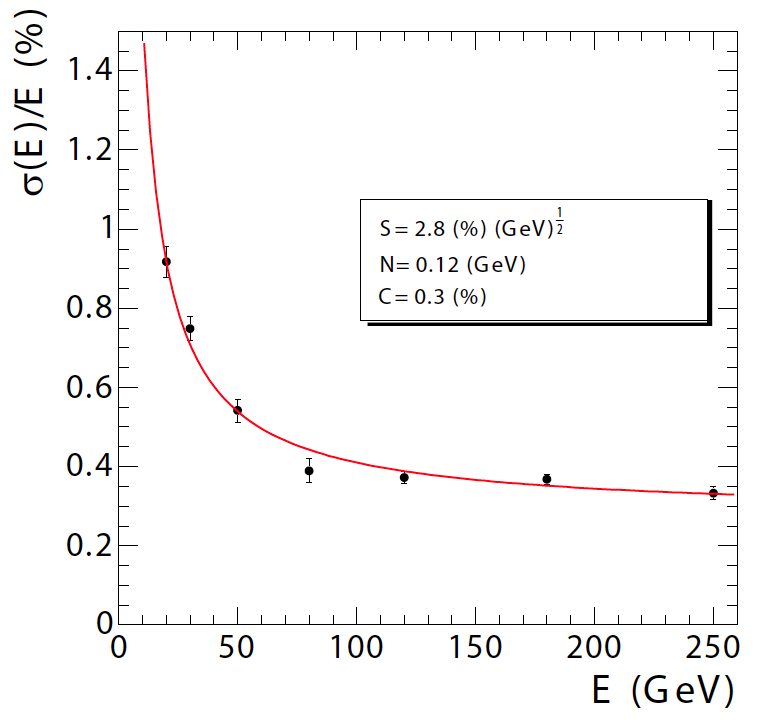
\includegraphics[width=0.6\textwidth]{tex/cms/fig/ecal-resolution.png}
  \caption{Energy resolution of the CMS ECAL as a function of electron energy as measured in a test beam.
    The fit (red) is parameterized by stochastic ($S$), noise ($N$), and constant ($S$) terms, as described
    in Equations \ref{eqn:ecal-resolution-1} and \ref{eqn:ecal-resolution-2} \cite{cms-jinst}.}
  \label{fig:ecal-resolution}
\end{figure}

